\documentclass[10pt, conference, compsocconf]{IEEEtran}
\usepackage{cite}
\usepackage{amsmath,amssymb,amsfonts}
\usepackage{algorithmic}
\usepackage{graphicx}
\usepackage{textcomp}
\usepackage[UTF8, heading = false, scheme = plain]{ctex}
\usepackage{pythonhighlight}
\hyphenation{op-tical net-works semi-conduc-tor}

\begin{document}

\title{加入中文支持的 IEEEtran 模板}

\author
{\IEEEauthorblockN{高睿昊}
    \IEEEauthorblockA
    {
    计算机科学与工程学院\\
    东南大学\\
    南京, 中国\\
    gaoruihao@wolf-tungsten.com
    }
}

\maketitle

\begin{abstract}
这里是摘要
\end{abstract}


\IEEEpeerreviewmaketitle

\section{项目}
\begin{itemize}
	\item	项目1
	\item	项目2

	
\end{itemize}

\section{第一部分}
这里是第一部分

\section{第二部分}
下面我们来插入一张图片
\begin{figure}[h]
	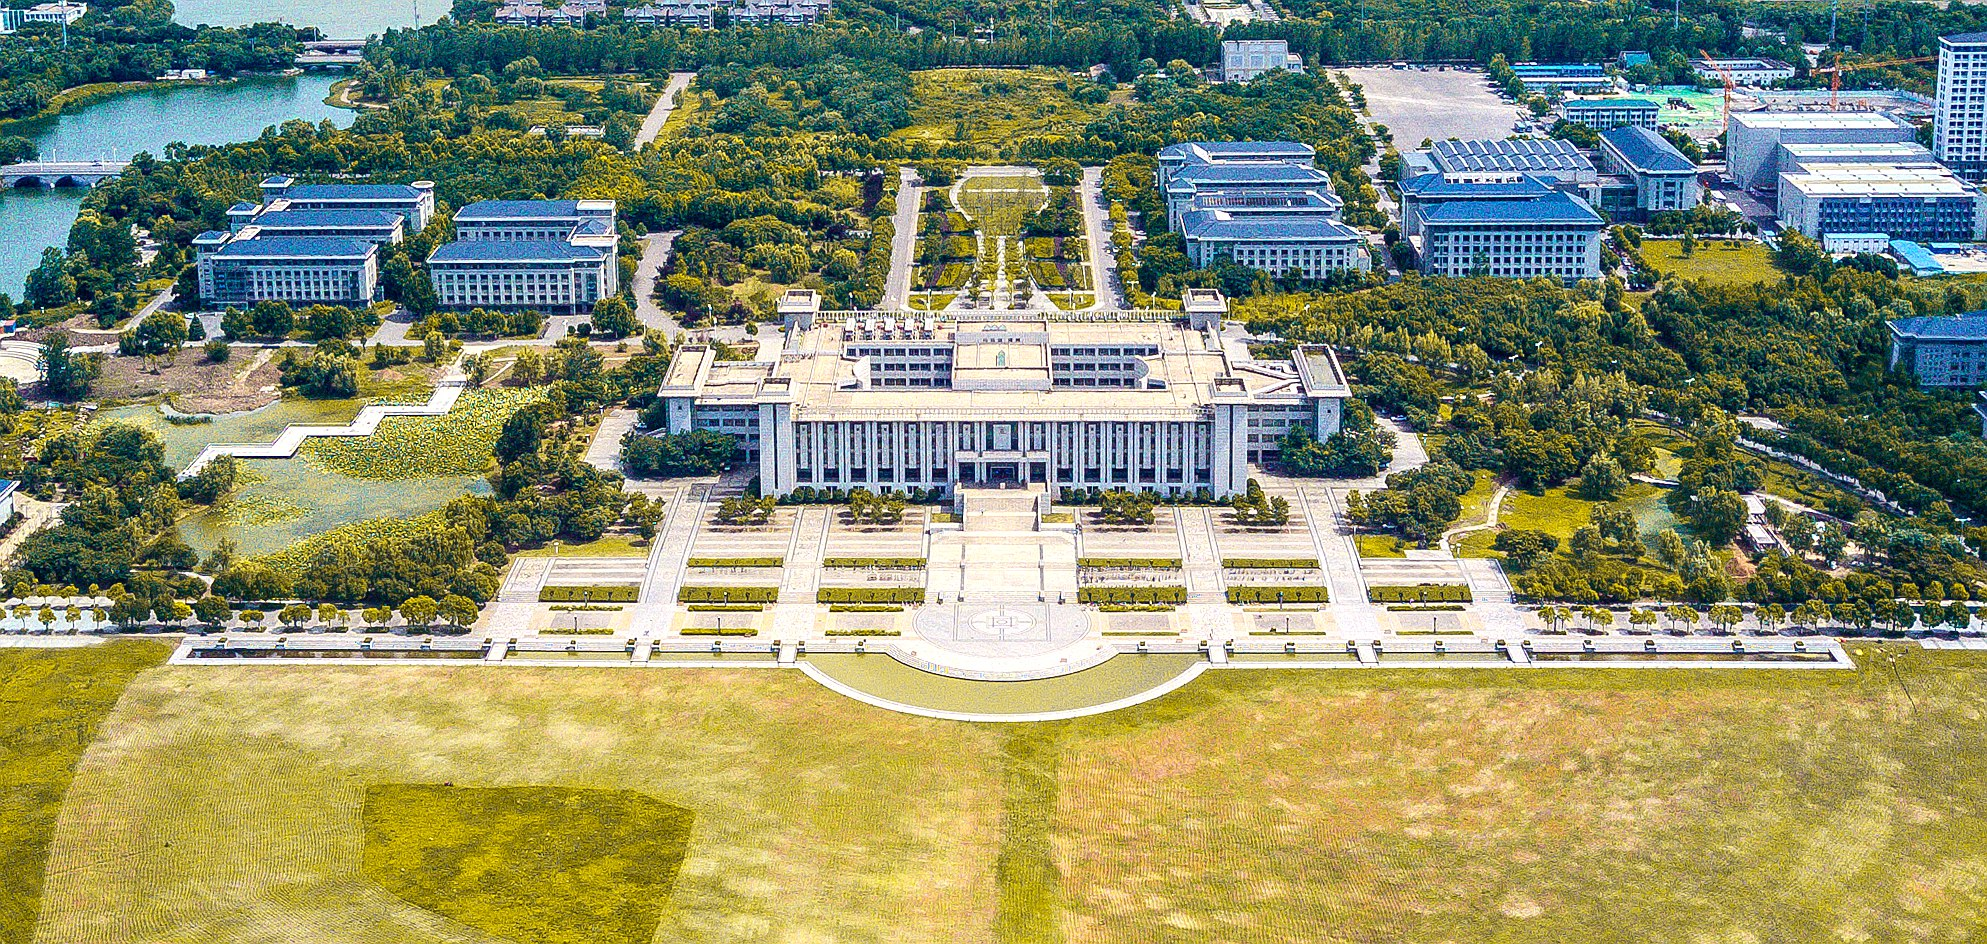
\includegraphics[width=8cm]{seu.jpg}
	\caption{东南大学} 
	\label{school}
\end{figure}


\subsection{小节}
可以导入代码
需要引用第三方库
\begin{python}
import numpy as np
a = np.random.randn((5,5))
\end{python}


\subsubsection{小小节}
我们来插入一个公式
\begin{equation}
  E= MC^2
\end{equation}


\begin{equation}
max(0,x)=\left\{
\begin{aligned}
0, \quad x \leq 0 & \\
1, \quad x > 0  &
\end{aligned}
\right.
\end{equation}

参考文献的引用:
\cite{yearbook2005china}

\bibliographystyle{IEEEtran} 
\bibliography{ref}   


\end{document}